\documentclass[11pt]{article}
\usepackage[utf8]{inputenc}
\usepackage[T1]{fontenc}
\usepackage{amsmath,amssymb}
\usepackage{graphicx}
\usepackage{booktabs}
\usepackage[margin=1in]{geometry}
\usepackage{hyperref}

\title{?`Que tan buena es la heuristica de independencia?\\
\large (Notebook: independence\_gap\_demo)}
\author{}
\date{}

\begin{document}
\maketitle

\begin{abstract}
El greedy dinamico usa una formula tipo producto sobre las marginales
$\tilde p_i$ para estimar cuantos infectados hay en un pool candidato
$t$. Esto asume que los $Z_i$ son independientes dado el historial, lo
cual en general NO es cierto. Este documento mide que tan lejos esta
esa heuristica de la probabilidad verdadera.

\textbf{Conclusion corta:} la mayoria del tiempo la heuristica acierta
(la mitad de los pools tienen error exactamente cero), pero en la cola
el error puede ser muy grande (hasta $0.55$).
\end{abstract}

%% ====================================================================
\section{?`Que estamos comparando?}

Cada individuo $i$ esta infectado ($Z_i = 1$) o no ($Z_i = 0$). Despues
de ver el historial $H$ (lista de pools probados y sus resultados),
el greedy mantiene las marginales posteriores
\[
\tilde p_i = \mathbb{P}(Z_i = 1 \mid H).
\]

Para decidir el siguiente pool, el greedy necesita saber cuantos
infectados hay en un pool candidato $t$, es decir la variable aleatoria
\[
r_t = \lvert t \cap Z \rvert = \sum_{i \in t} Z_i.
\]

El greedy aproxima la distribucion de $r_t$ asumiendo que los $Z_i$ son
independientes dado $H$. Con esa suposicion, $r_t$ tiene una distribucion
Poisson-Binomial con parametros $(\tilde p_i)_{i \in t}$. En particular:
\begin{itemize}
  \item $\mathbb{P}(r_t = 0 \mid H) \approx \prod_{i \in t} (1 - \tilde p_i)$
    (el caso "clear" que usa el score myopico).
  \item $\mathbb{P}(r_t = \lvert t \rvert \mid H) \approx \prod_{i \in t} \tilde p_i$
    (el caso "todos infectados", que es la formula que escribe el usuario).
\end{itemize}

\textbf{El problema:} tests previos introducen dependencias entre los
$Z_i$. Por ejemplo, si antes probamos $t' \subsetneq t$ y $t'$ salio
positivo (al menos un infectado), entonces $t$ tambien tiene al menos
un infectado con probabilidad 1. Pero la heuristica le sigue dando masa
positiva al evento "ningun infectado en $t$".

%% ====================================================================
\section{Ejemplo concreto}

Cuatro personas con prior $p_i = 0.5$. Historial: probamos $t' = \{0,1\}$
y el resultado fue $r' = 1$ (exactamente uno de los dos esta infectado).
Ahora miramos el pool $t = \{0,1,2,3\}$.

Como al menos uno de $\{0,1\}$ esta infectado, se sigue que $r_t \ge 1$
siempre, es decir, $\mathbb{P}(r_t = 0 \mid H) = 0$ exacto.

Pero las marginales posteriores de $0$ y $1$ son $\tilde p_0 = \tilde p_1 = 0.5$
(por simetria), asi que la heuristica da
\[
\prod_{i \in t}(1 - \tilde p_i) = 0.5 \cdot 0.5 \cdot 0.5 \cdot 0.5 = 0.0625.
\]

\begin{table}[h]
\centering
\begin{tabular}{lccccc}
\toprule
 & $r_t=0$ & $r_t=1$ & $r_t=2$ & $r_t=3$ & $r_t=4$ \\
\midrule
Exacta      & 0.0000 & 0.2500 & 0.5000 & 0.2500 & 0.0000 \\
Heuristica  & 0.0625 & 0.2500 & 0.3750 & 0.2500 & 0.0625 \\
\bottomrule
\end{tabular}
\caption{Distribucion exacta de $r_t$ vs. la heuristica Poisson-Binomial.
El error en los extremos es $0.0625$; la distancia de variacion total es $0.125$.}
\end{table}

Interesante: las marginales son correctas (cada $\tilde p_i$ es exacto),
pero la forma de la distribucion esta mal porque los $Z_i$ no son
independientes una vez vista la historia.

%% ====================================================================
\section{?`Que tan frecuente es esto?}

Generamos 300 instancias aleatorias con $n = 8$ personas, priors
uniformes en $[0.05, 0.5]$, y 3 tests seleccionados con el greedy
myopico. Para cada instancia evaluamos \emph{todos} los pools
candidatos de tamano 2 y 3, y comparamos la distribucion exacta
(por enumeracion de los $2^n$ mundos) contra la heuristica
Poisson-Binomial.

Medimos tres cosas por pool:
\begin{itemize}
  \item \textbf{TV} (distancia de variacion total): suma de las
    diferencias absolutas entre las dos PMFs, dividida entre 2.
    Va de 0 (igual) a 1 (totalmente distinto).
  \item \textbf{Error en "ninguno infectado"}:
    $\big\lvert \mathbb{P}(r_t=0 \mid H) - \prod (1-\tilde p_i) \big\rvert$.
  \item \textbf{Error en "todos infectados"}:
    $\big\lvert \mathbb{P}(r_t=\lvert t \rvert \mid H) - \prod \tilde p_i \big\rvert$.
\end{itemize}

\begin{table}[h]
\centering
\begin{tabular}{lrrrrrrr}
\toprule
$\lvert t \rvert$ & n pools & TV media & TV mediana & TV p95 & TV max & gap r0 medio & gap rmax medio \\
\midrule
2 & 8400 & 0.0243 & 0.0000 & 0.2166 & 0.5000 & 0.0121 & 0.0121 \\
3 & 16800 & 0.0501 & 0.0000 & 0.4696 & 0.5555 & 0.0238 & 0.0091 \\
\bottomrule
\end{tabular}
\caption{Error de la heuristica sobre 300 instancias ($n=8$, $B=3$, $G=3$).
La mediana es cero: la mayoria del tiempo la heuristica acierta.
Pero el p95 y el max muestran que la cola es gorda.}
\end{table}

\textbf{Lectura:}
\begin{itemize}
  \item En mas de la mitad de los pools, el error es cero: la
    heuristica acierta. Esto pasa cuando el pool no se traslapa con
    el historial, o cuando todo el pool ya quedo determinado por los
    tests previos.
  \item En el top 5\% de los pools (la "cola"), el error llega hasta
    $\sim 0.47$ para pools de tamano 3: errores grandes.
  \item El peor caso ($\sim 0.55$) aparece cuando el historial
    "amarra" a un subconjunto del pool (como en el ejemplo de arriba)
    pero deja las marginales individuales intermedias.
\end{itemize}

\begin{figure}[h]
\centering
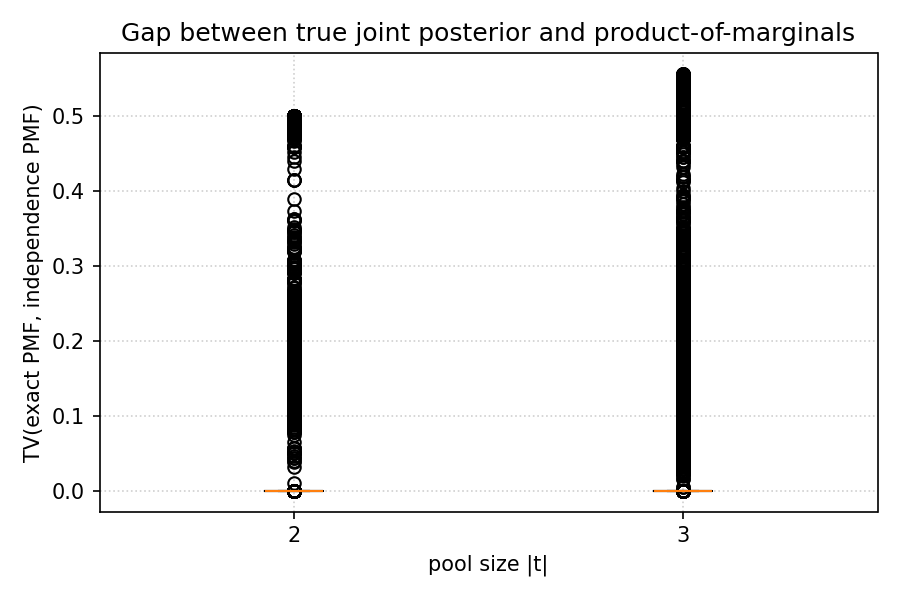
\includegraphics[width=0.85\textwidth]{paper_figs/independence_gap_tv_by_size.png}
\caption{Error entre la PMF exacta y la heuristica, agrupado por
tamano del pool. La caja esta pegada a cero: la mayoria de los pools
tiene error muy pequeno. Los puntos sueltos arriba son casos raros
donde el error llega casi a $0.55$.}
\end{figure}

\begin{figure}[h]
\centering
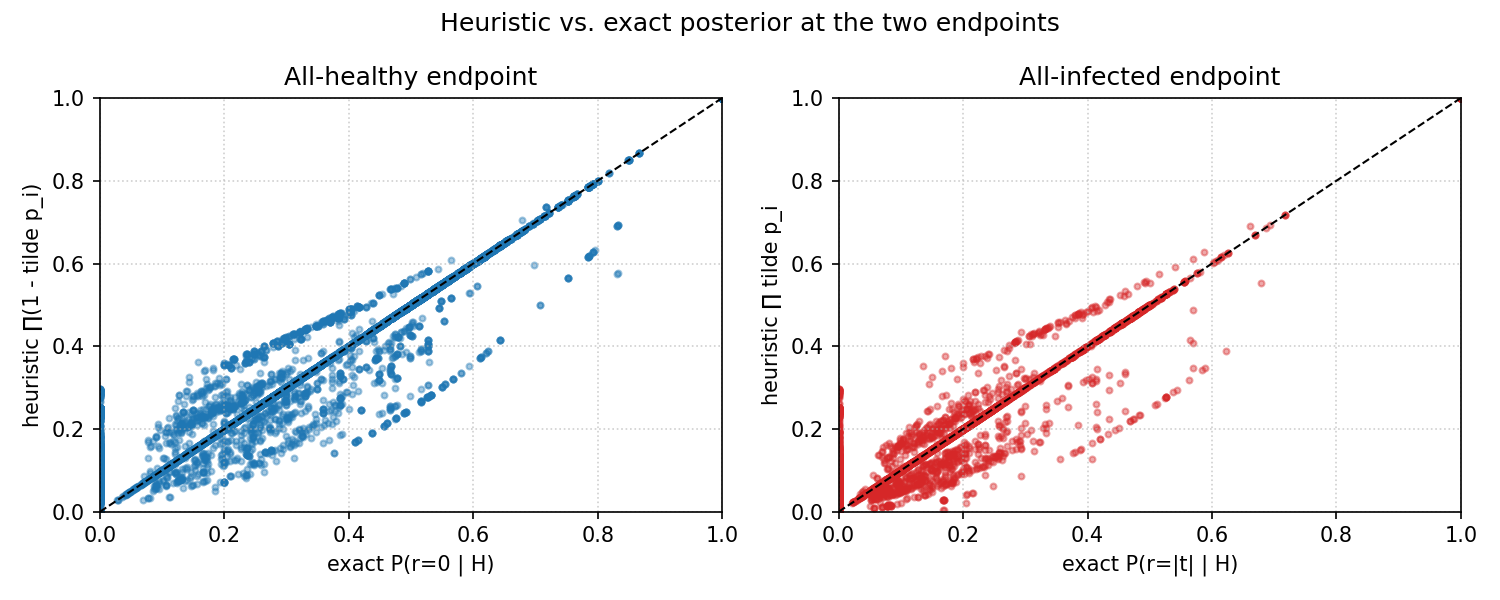
\includegraphics[width=0.85\textwidth]{paper_figs/independence_gap_endpoints.png}
\caption{Cada punto es un pool. A la izquierda comparamos la
probabilidad de "ninguno infectado": eje x la exacta, eje y la
heuristica. A la derecha, "todos infectados". La linea punteada es la
diagonal (heuristica $=$ exacta). La mayoria cae sobre la diagonal,
pero hay una nube sobre la diagonal a la izquierda: la heuristica a
veces dice que el pool puede "limpiar" cuando en realidad el historial
ya excluye ese evento.}
\end{figure}

%% ====================================================================
\section{?`Cuando falla la heuristica?}

Los 5 peores casos del experimento comparten el mismo patron:
$\mathbb{P}(r_t = 0 \mid H) = 0$ exactamente (el historial garantiza al
menos un infectado en $t$), pero la heuristica da masa entre $0.03$ y
$0.30$ ahi. Ese error se "contagia" al resto de la PMF porque los
$\tilde p_i$ son correctos pero ignoran la correlacion.

En concreto, el error de la heuristica aumenta cuando:
\begin{enumerate}
  \item Hay un $t' \subsetneq t$ en la historia con $0 < r' < \lvert t' \rvert$
    (resultado intermedio: amarra a los miembros sin determinarlos).
  \item Varios pools del historial se traslapan con $t$ (mas
    restricciones conjuntas no capturadas por las marginales).
  \item El tamano del pool candidato es mayor (mas productos de
    marginales que acumulan el error).
\end{enumerate}

Cuando la historia \emph{si} determina a todos los miembros del pool
(por ejemplo, un test con $r' = 0$ o $r' = \lvert t' \rvert$ sobre
todo el pool), las $\tilde p_i$ son $0$ o $1$ y la heuristica recupera
exactamente la distribucion verdadera. Cuando la historia no toca al
pool, tambien coinciden. Esos dos casos dominan la muestra y por eso
la mediana del error es cero. El problema aparece en el medio: cuando
la historia amarra a \emph{algunos} miembros sin determinarlos.

%% ====================================================================
\section{Implicaciones para el greedy}

El score myopico es
\[
\text{score}(t) = \mathbb{P}(r_t = 0 \mid H) \cdot \sum_{i \in t} u_i,
\]
pero se computa con la heuristica
$\prod_{i \in t}(1 - \tilde p_i)$. Cuando esa probabilidad heuristica
esta sobreestimada (como en los peores casos aqui), el greedy puede
preferir pools que en realidad NUNCA van a "limpiar" nada.

Una direccion razonable es:
\begin{itemize}
  \item Reemplazar $\prod (1 - \tilde p_i)$ por la probabilidad exacta
    $\mathbb{P}(r_t = 0 \mid H)$, calculada directamente sobre la
    distribucion conjunta (por ejemplo, con el counting ya implementado
    o una consulta conjunta via Gibbs).
  \item Medir si esa correccion reduce la brecha contra el optimo,
    usando los mismos experimentos de phase3/sprint3.
\end{itemize}

%% ====================================================================
\section{Como reproducir}

\begin{verbatim}
python augmented/independence_gap_demo.py
\end{verbatim}

Los tests unitarios estan en \texttt{augmented/tests.py}
(prefijos \texttt{test\_exact\_pool\_pmf\_...},
\texttt{test\_deterministic\_subset\_...}, etc.) y la logica esta en
\texttt{augmented/independence\_gap.py}.

\end{document}
